\documentclass{article}
\usepackage{ctex} % 加入ctex宏包以支持中文
\usepackage{graphicx} % 用于插入图片
\usepackage{geometry} % 用于设置页面布局
\usepackage{booktabs} % 用于美化表格
\usepackage{enumitem} % 用于自定义列表格式
\usepackage{lipsum}  % 导入生成段落的宏包
\usepackage{ctex} % 加入ctex宏包以支持中文
\usepackage{graphicx} % 加载图形处理宏包
\usepackage{booktabs} % 用于美化表格线条
\usepackage{caption} % 用于添加表格标题
\usepackage[table]{xcolor} % 用于设置表格颜色
\usepackage{float}
\usepackage{tabularx}
\usepackage{tcolorbox}
\tcbuselibrary{listings}
\usepackage{array}
\usepackage[dvipsnames]{xcolor}
\usepackage{tikz}
\usepackage{hyperref} 
\usetikzlibrary{positioning} % 加载positioning库
\renewcommand{\refname}{Reference}

\hypersetup{
    colorlinks=true, % 使用颜色而不是边框
    linkcolor=black, % 链接颜色为黑色
    citecolor=black, % 引用颜色为黑色
    urlcolor=blue    % URL颜色为蓝色(可以根据需要修改)
}
\lstset{
 basicstyle=\ttfamily, % 设置字体族
 breaklines=true, % 自动换行
 keywordstyle=\bfseries\color{NavyBlue}, % 设置关键字为粗体,颜色为 NavyBlue
 morekeywords={}, % 设置更多的关键字,用逗号分隔
 emph={self}, % 指定强调词,如果有多个,用逗号隔开
    emphstyle=\bfseries\color{Rhodamine}, % 强调词样式设置
    commentstyle=\itshape\color{black!50!white}, % 设置注释样式,斜体,浅灰色
    stringstyle=\bfseries\color{PineGreen!90!black}, % 设置字符串样式
    columns=flexible,
    % numbers=left, % 显示行号在左边
    % numbersep=2em, % 设置行号的具体位置
    % numberstyle=\footnotesize, % 缩小行号
    frame=single, % 边框
    framesep=1em, % 设置代码与边框的距离
	tabsize=2, % 设置tab键的宽度为2个空格
    showstringspaces=false, % 不显示字符串中的空格
}

\geometry{a4paper, margin=1in}
\begin{document}

\begin{titlepage}
    \centering
    \vspace*{1cm}

    % 插入学校标志
    
\includegraphics[width=\textwidth]{img/logo.png} % 假设logo.png是学校标志的图片文件

    % \vspace{1.5cm}
    \fontsize{24pt}{32pt}\selectfont
    \textbf{《High-level Language Programming Project》 Report}
    \vspace{6cm}

    \fontsize{20pt}{20pt}\selectfont
    \begin{tabular}{ll}
        Project Name:    & Ztest: A C++ Unit Testing Framework \\
                         &                                     \\
        School       :   & \hspace{6cm}                        \\
        Major        :   & \hspace{6cm}                        \\
        Student Name :   & \hspace{6cm}                        \\
        Teacher      :   & \hspace{6cm}                        \\
        Submission Date: & \hspace{6cm}                        \\
    \end{tabular}

    \vfill

    \vspace{1cm}
\end{titlepage}

\tableofcontents  % 生成目录表
\newpage
\section{系统需求分析}
\subsection{系统背景与动机}
% 在这里填写系统背景和动机的内容
随着复杂系统架构设计能力的培养需求日益凸显,掌握面向对象设计原则与模式化工程实践已成为高级软件工程教育的核心目标。这不仅需要理解类与对象间的动态协作关系,更要具备通过设计模式解决架构难题的抽象思维能力。
现有的单元测试框架(如Google Test)具有上手难度较高,并发支持有限,报告系统过于简洁,可拓展性一般等缺点,我们团队计划开发一个提供一个灵活、高效且易于使用(带图形用户界面GUI)的测试工具,旨在提供一个直观、易用的环境,方便开发人员和测试人员编写、运行和管理测试用例。该工具将支持多种测试类型(如单元测试、集成测试等),并提供详细的测试结果报告。
\begin{table}[h]
    \centering
    \caption{主流测试框架对比}
    \label{tab:compare}
    \begin{tabularx}{\textwidth}{lXXXXX}
        \toprule
        \textbf{框架}              & \textbf{GUI支持} & \textbf{并发测试} & \textbf{报告系统} & \textbf{扩展性} & \textbf{数据驱动} \\
        \midrule
        Google Test(C++)         & 无              & 有限            & 基础            & 中等           & 不支持           \\
        JUnit    (Java)          & Eclipse插件      & 支持            & HTML/XML      & 高            & 支持            \\
        PyTest (Python)          & 第三方工具          & 优秀            & 丰富            & 优秀           & 支持            \\
        Catch2   (C++)           & 无              & 一般            & 简洁            & 中等           & 不支持           \\
        % \midrule
        \textbf{Ztest*}    (C++) & 精美             & 优秀            & 丰富            & 高            & 支持            \\
        \bottomrule
    \end{tabularx}
\end{table}
\subsection{系统目标}
\begin{figure}[H]
    \centering
    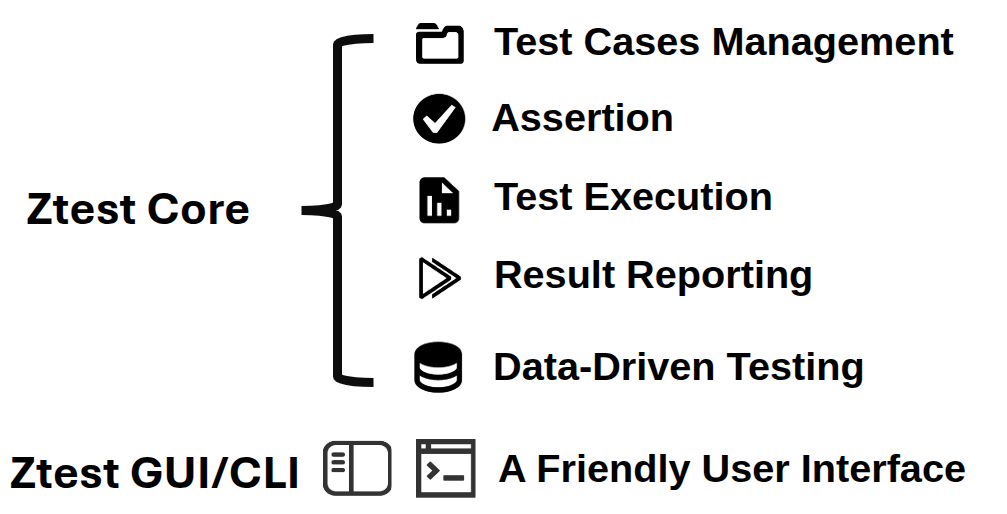
\includegraphics[width=0.6\textwidth]{img/func.png} % 假设logo.png是学校标志的图片文件
    \caption{ ztest function}
    \label{fig:ztest function }
\end{figure}
\subsubsection{测试管理}
% 我们将任务分为四个类别:短测试时间且更关注结果正确性的任务,如加法运算、字符串拼接和用户登录验证;长测试时间且更关注结果正确性的任务,如合并多个文件、复杂字符串匹配与替换和大量数据排序结果验证;短测试时间且更关注运行过程评估的任务,如读取或写入大文件、低复杂度算法性能测试和数据库查询;以及长测试时间且更关注运行过程评估的任务,如多线程处理任务、压力测试和时间复杂度高算法测试。

% \begin{figure}[H]
%     \centering
%     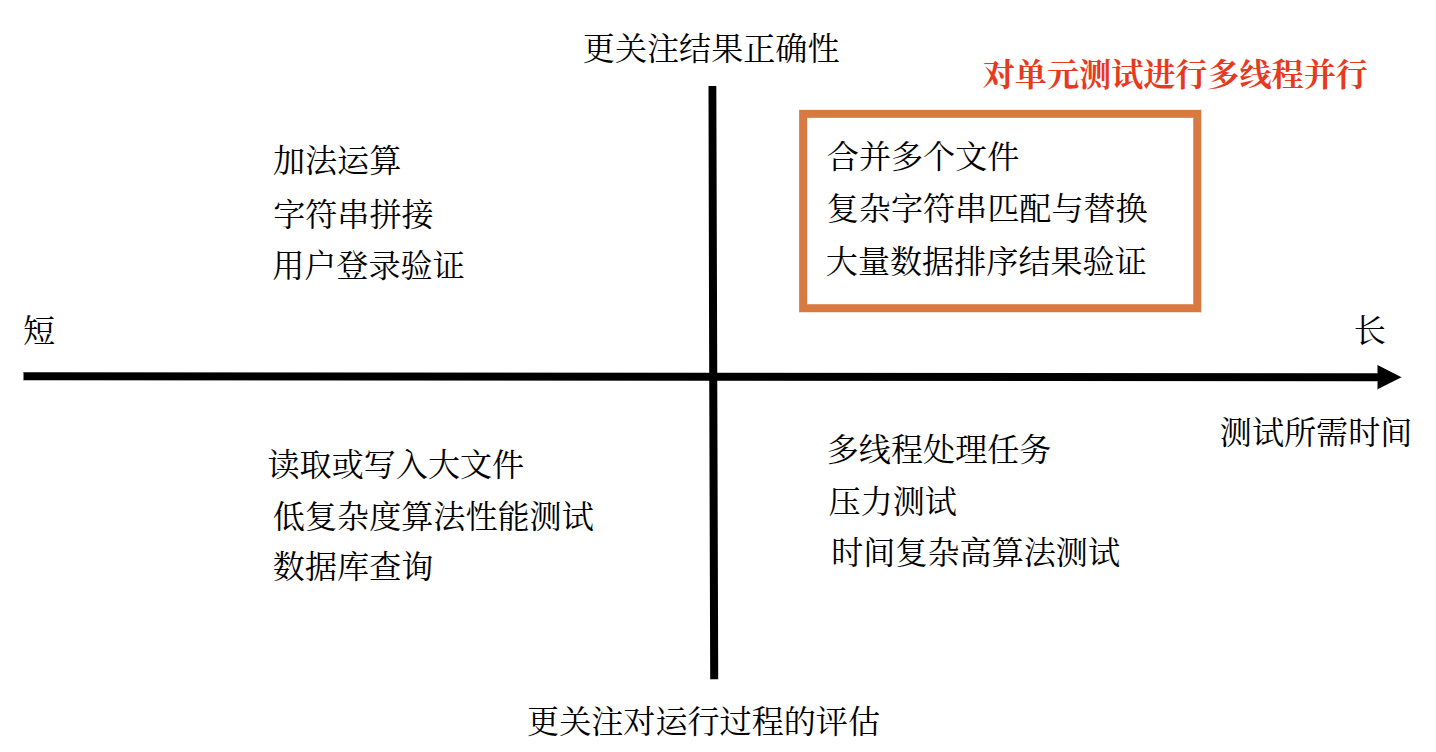
\includegraphics[width=0.6\textwidth]{img/task.png} % 假设logo.png是学校标志的图片文件
%     \caption{ task type}
%     \label{fig:ztest task type }
% \end{figure}

相较传统的单元测试框架,Ztest支持多种测试类型,如可并行运行且线程安全测试、需串行运行或线程不安全测试、通过迭代评估性能、参数化数据驱动测试。我们提供测试夹具用来管理单个测试。

\begin{figure}[H]
    \centering
    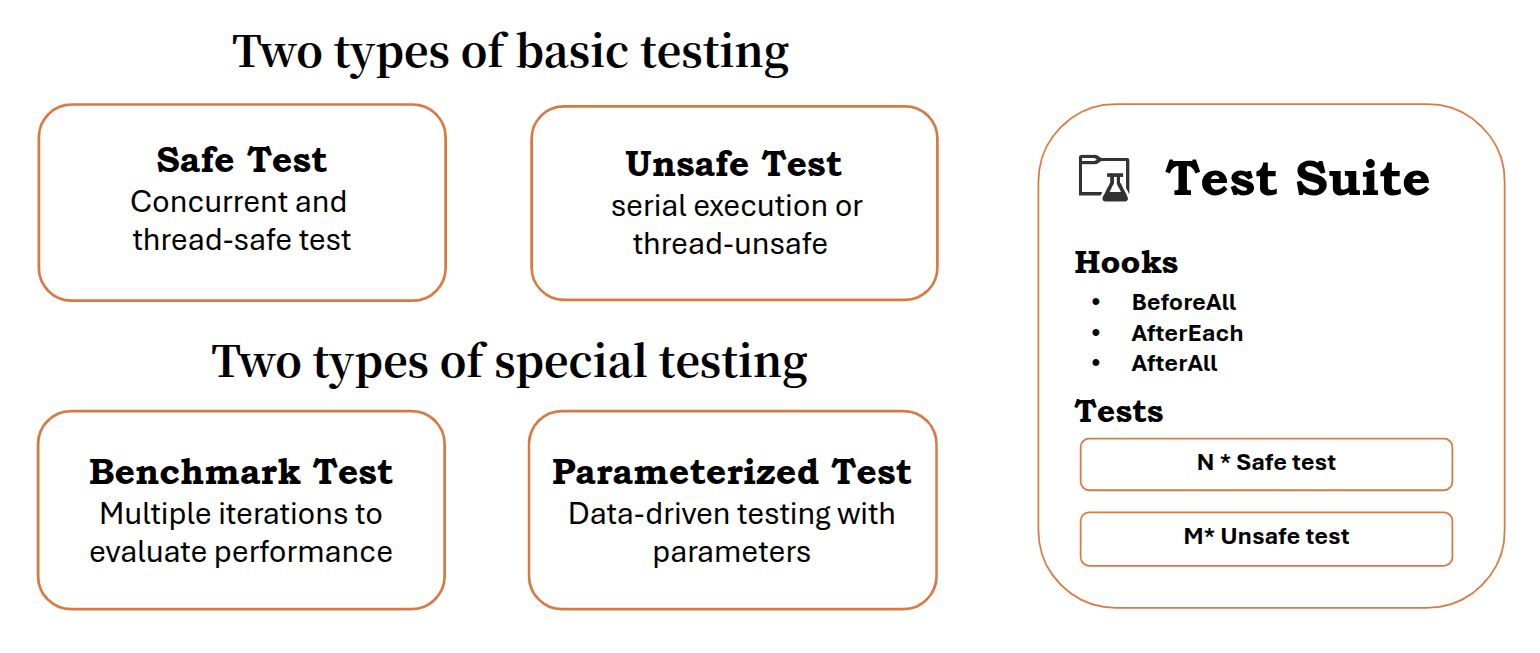
\includegraphics[width=0.8\textwidth]{img/types.png} % 假设logo.png是学校标志的图片文件
    \caption{ test type}
    \label{fig:test types }
\end{figure}
我们提供类似Google Test的宏简化测试定义:
\begin{lstlisting}[language=C++]
ZTEST_F(SuiteName, TestName, safe/unsafe) { ... } //define a test 
ZBENCHMARK(SuiteName, TestName, iterations) { ... } // define a benchmark
ZTEST_P(SuiteName, TestName, data) { ... }  //define a parameterized test
ZTEST_P_CSV(SuiteName, TestName, "data.csv") { ... } // define a parameterized test with csv data
\end{lstlisting}

同时,我们能够链式定义测试用例:
\begin{lstlisting}[language=C++]
auto test_case = TestFactory::createTest("Add", ZType::Z_SAFE, "", add, 2, 3)
                 .setExpectedOutput(5)
                 .beforeAll([]() { logger.info("Init\n"); })          
                 .afterEach([]() { logger.info("Clean\n"); }).build();
                \end{lstlisting}
\subsubsection{断言机制}
断言机制用于验证测试用例的预期结果是否正确。框架提供了多种断言宏,如 \textbf{EXPECT\_EQ} 和 \textbf{ASSERT\_TRUE},支持在测试中快速验证条件。
主要提供以下断言:
\begin{itemize}
    \item \textbf{EXPECT\_EQ}:验证两个值是否相等。
    \item \textbf{ASSERT\_TRUE}:验证条件是否为真。
\end{itemize}
使用样例如下,
\begin{lstlisting}[language=C++]
// 如果断言失败,抛出异常
EXPECT_EQ(5, add(2, 3));
ASSERT_TRUE(6==add(2, 3));
\end{lstlisting}

如果断言失败,抛出 \textbf{ZTestFailureException} 异常。同时可以通过继承 \textbf{ZTestFailureException} 异常处理函数,自定义异常处理逻辑。
\subsubsection{数据驱动测试}
参数化测试是指在测试过程中,将测试用例中某些固定的数据替换为参数,然后通过改变参数的值来生成多组测试数据,从而对软件进行多次测试的方法。它允许测试人员用一组测试逻辑覆盖多种输入情况,而不是为每种情况编写单独的测试代码。
数据驱动测试框架(Data-Driven Testing Framework)是一种将测试数据与测试脚本分离的自动化测试框架。它通过外部数据源(如Excel、CSV文件、数据库等)来驱动测试用例的执行。

ZTest实现了参数测试并以从csv导入和解析数据的方式实现了数据驱动的测试。为了加速数据的访问,缓存导入的数据。使用懒加载机制,只有在需要时才加载数据到缓存中,减少不必要的资源消耗。同时,使用了LRU缓存淘汰策略用来确保缓存中的数据是最有可能被再次访问的,从而最大限度地发挥缓存的作用。

\subsubsection{测试执行器}
测试执行器负责管理测试用例的运行,支持\textbf{多线程}并行执行测试用例,并收集测试结果,实现了自动调度测试和测试结果统计。
他的行为如下:
\begin{itemize}
    \item 并行运行safe测试。线程的创建和销毁是一个相对耗时的操作。使用线程池管理线程的生命周期通过复用线程,避免了频繁的线程创建和销毁,从而显著提高了系统的性能。
    \item 串行运行unsafe测试。通过队列来维护测试用例,保证测试用例的顺序执行。
    \item 串行运行Benchmark测试。
    \item 串行运行Parameterized测试。
\end{itemize}
\subsubsection{报告生成}
能够生成HTML,JSON和XML报告,方便查看测试结果和用于CI/CD。
\begin{figure}[H]
    \centering
    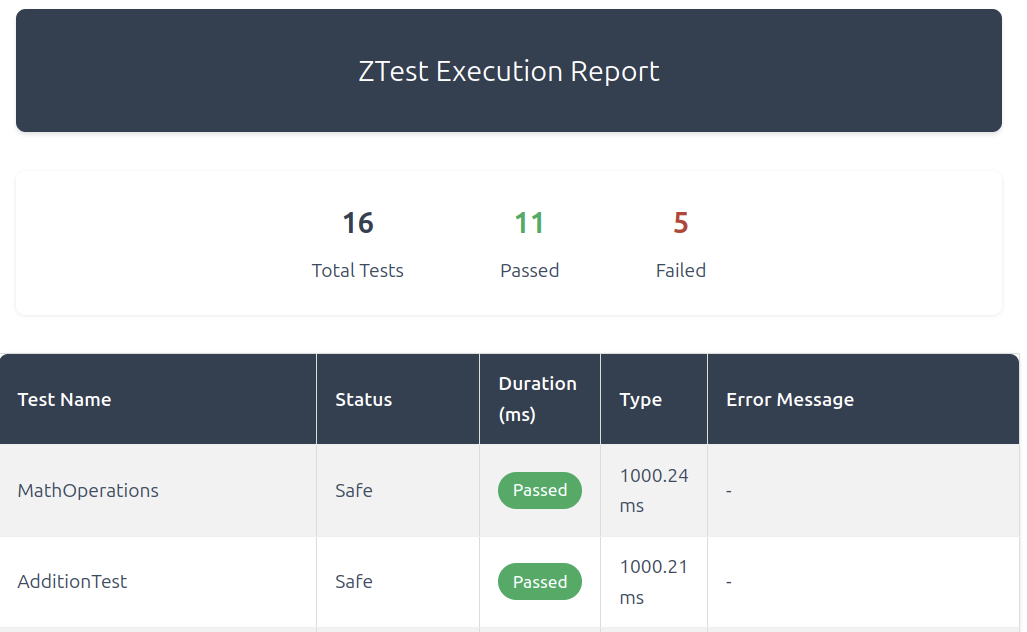
\includegraphics[width=0.8\textwidth]{img/report.png}
    \caption{测试结果展示界面布局示意图}
    \label{fig:report}
    \small
\end{figure}
\subsubsection{CLI接口}
\begin{lstlisting}
Usage: executor_name [OPTIONS] 
Options: 
--help                         Show help 
--run-all                      Run all tests
--run-safe                     Run safe tests
--run-unsafe                   Run unsafe tests
--run-benchmark                Run benchmark tests
--run-parameterized            Run parameterized tests
--run-test-case TEST_CASE      Run a specific test case
\end{lstlisting}

\subsubsection{GUI展示}
可以通过GUI展示测试结果,筛选测试结果,观看系统资源状态,查看某个测试的运行细节等功能。
\begin{figure}[H]
    \centering
    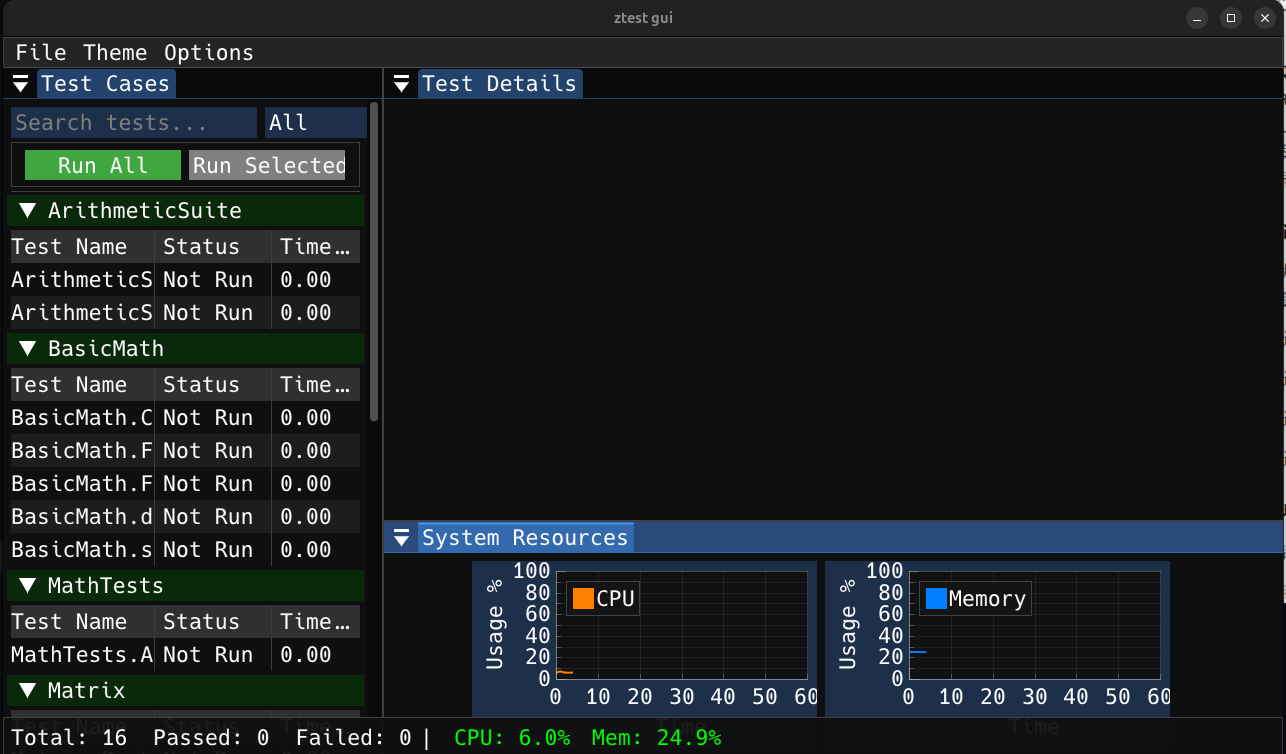
\includegraphics[width=\textwidth]{img/gui.png}
    \caption{测试管理界面布局示意图}
    \label{fig:gui}
    \small
\end{figure}

\newpage
\section{程序分析}
\subsection{ 系统关键问题}
\subsubsection{提升测试运行效率}
传统的C++测试框架(如gtest,catch2)多使用顺序运行测试的方法执行所有测试,导致测试时间较长,降低了生产效率。同时vibe coding的出现导致编写测试用例的时间大大降低,而运行测试用例的时间仍然没有大的降低。
我们将任务分为四个类别:短测试时间且更关注结果正确性的任务,如加法运算、字符串拼接和用户登录验证;长测试时间且更关注结果正确性的任务,如合并多个文件、复杂字符串匹配与替换和大量数据排序结果验证;短测试时间且更关注运行过程评估的任务,如读取或写入大文件、低复杂度算法性能测试和数据库查询;以及长测试时间且更关注运行过程评估的任务,如多线程处理任务、压力测试和时间复杂度高算法测试。
\begin{figure}[H]
    \centering
    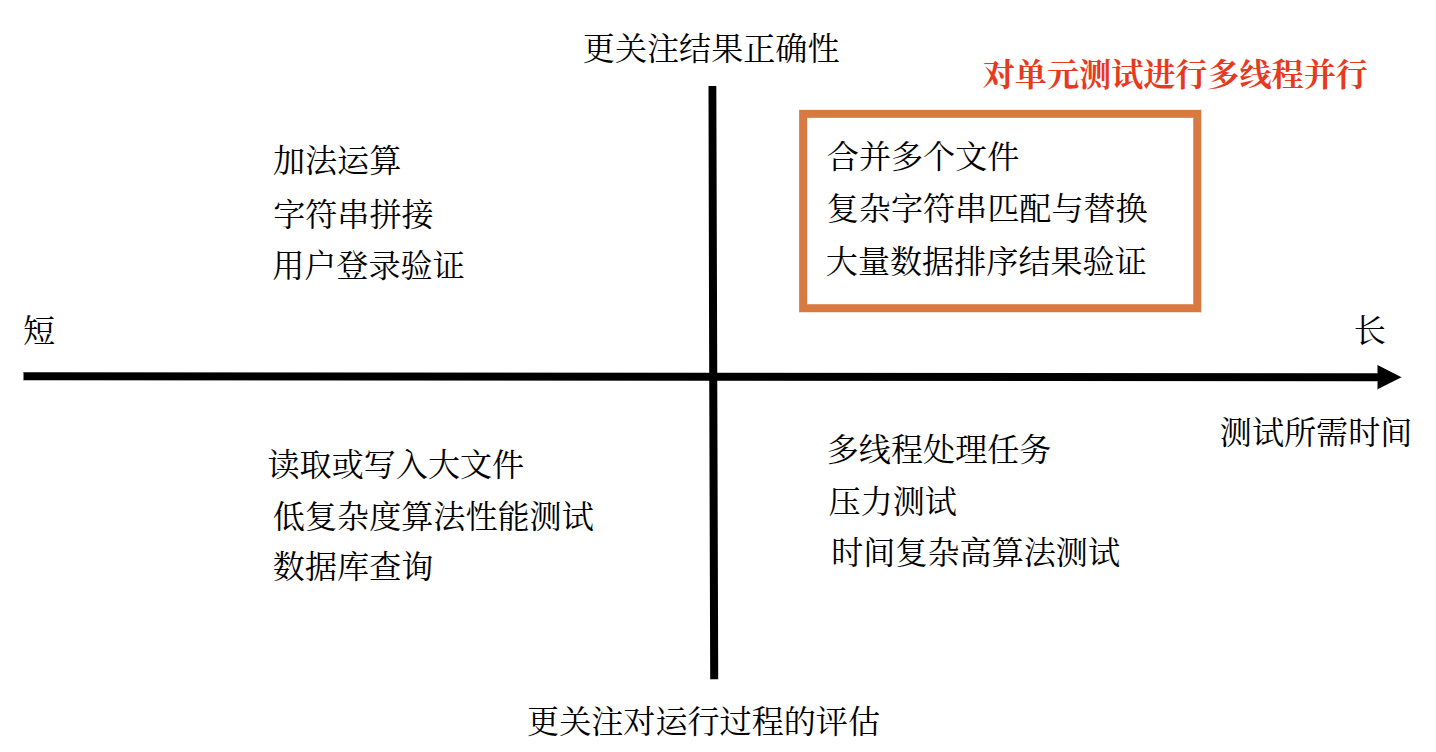
\includegraphics[width=0.8\textwidth]{img/task.png} % 假设logo.png是学校标志的图片文件
    \caption{ task type}
    \label{fig:task types }
\end{figure}
对于测试所需时间长,更见关注结果正确性,且线程安全的任务,ZTest从pytest中借鉴,在C++测试框架体系中引入了多线程测试执行。截至目前,没有任意一个主流C++单元测试引入了这一机制。
同时,引入数据驱动测试并使用缓存加速使得大规模的单元测试的定义和执行速度大大提升,意义重大。
\subsubsection{语法糖的实现}
如何让用户愿意使用单元测试框架?其关键在于语法定义的简易性。我们使用一系列复杂的宏定义来实现语法糖,从而简化用户的定义。
\subsubsection{待测函数的自动类型推导}
我们设计在使用单个测试样例链式定义的时候,我们希望用户只需要传入函数名、参数和期望结果,就可以由为我们的框架接管运行的具体逻辑和测试结果的比较。
这要求我们实现自动推导待测函数的参数类型,以便调用函数用于测试和测试结果验证。我们使用工厂模式来实现返回值类型的指定,使用建造者模式来实现参数的构造和期望结果的设定。
\subsection{ 职责分配}
% 在这里填写每个学生的职责分配
\begin{itemize}[leftmargin=*]
    \item 学生1: [任务1]
    \item 学生2: [任务2]
    \item 学生3: [任务3]
          % 根据实际情况继续添加
\end{itemize}

\section{技术路线}
\subsection{运行环境}
\begin{table}[H]
    \centering
    \caption{开发和运行环境}
    \begin{tabular}{@{}>{\bfseries}c>{\raggedright\arraybackslash}p{10cm}@{}} % 设置第一列为加粗,第二列为左对齐
        \toprule
        \textbf{Component} & \textbf{Tool Used for Development}                    \\
        \midrule
        处理器                & Intel i9-14900HX (32) @ 5.800GHz                      \\
        操作系统               & Ubuntu 24.04.2 LTS x86\_64 (kernel 6.11.0-26-generic) \\
        编译器                & gcc 13.3.0 或 clang 18.1.3 (不可以使用MSVC)                 \\
        图形API              & glfw 3.4 + glad 4.0.1                                 \\
        GUI框架              & ImGui-1.91.7-docking                                  \\
        数据可视化工具            & implot v0.16                                          \\
        构建系统               & XMake v2.9.9+HEAD.40815a0                             \\
        C++标准              & C++20(必要)                                             \\
        \bottomrule
    \end{tabular}
\end{table}
\subsection{总体设计}
\subsubsection{Ztest Core架构图}
% 在这里描述系统的总体设计
\begin{figure}[H]
    \centering
    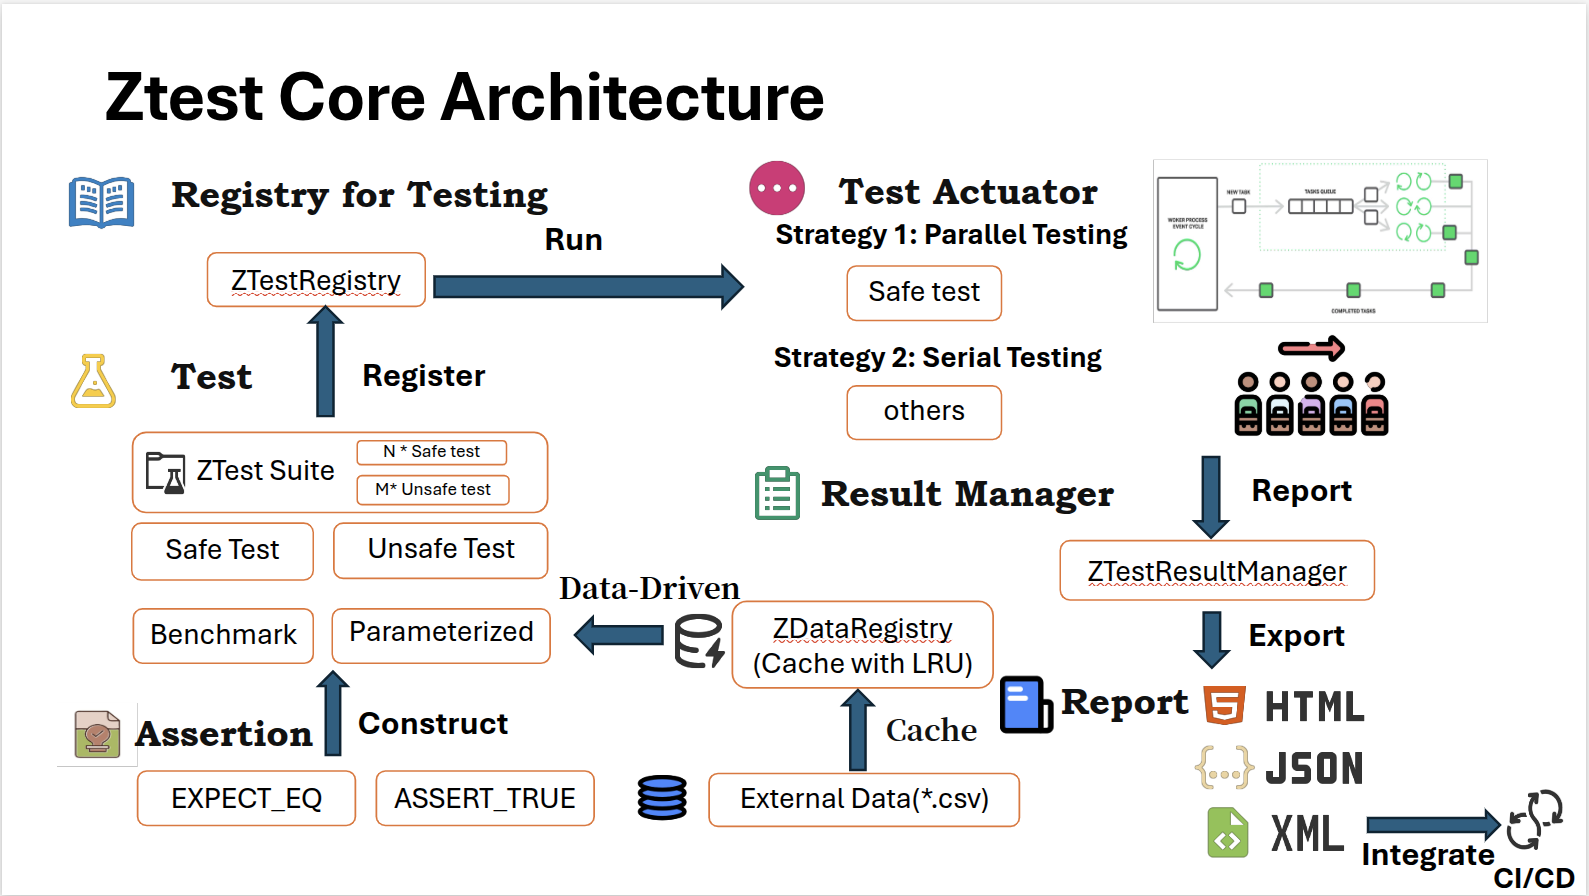
\includegraphics[width=0.8\textwidth]{img/corearch.png} % 假设logo.png是学校标志的图片文件
    \caption{ ztest design}
    \label{fig:ztest design }
\end{figure}
ZTest的核心架构流程开始于测试定义阶段,测试(包括ZTest Suite、安全测试、不安全测试、基准测试和参数化测试)通过会使用断言定义,如EXPECT\_EQ和ASSERT\_TRUE,来验证测试结果的正确性。
接着,测试将被注册到ZTestRegistry进行统一的管理。
注册完成后,测试会被发送到测试执行器,该执行器根据测试的类型采取不同的测试策略,对于安全测试采用并行测试策略,而对于其他类型的测试则采用串行测试策略。
在对数据驱动的测试的执行过程中,数据驱动模块通过ZDataRegistry(带有LRU机制的缓存)来管理外部数据,如CSV文件,以支持测试的进行。
测试完成后,结果管理器ZTestResultManager负责收集和处理测试结果,并将这些结果导出为HTML、JSON或XML格式,以便于报告和进一步分析。
此外,整个测试流程还支持与持续集成/持续部署(CI/CD)系统的集成,使得测试结果可以自动地反馈到开发流程中,从而提高软件开发的效率和质量。
\begin{figure}[H]
    \centering
    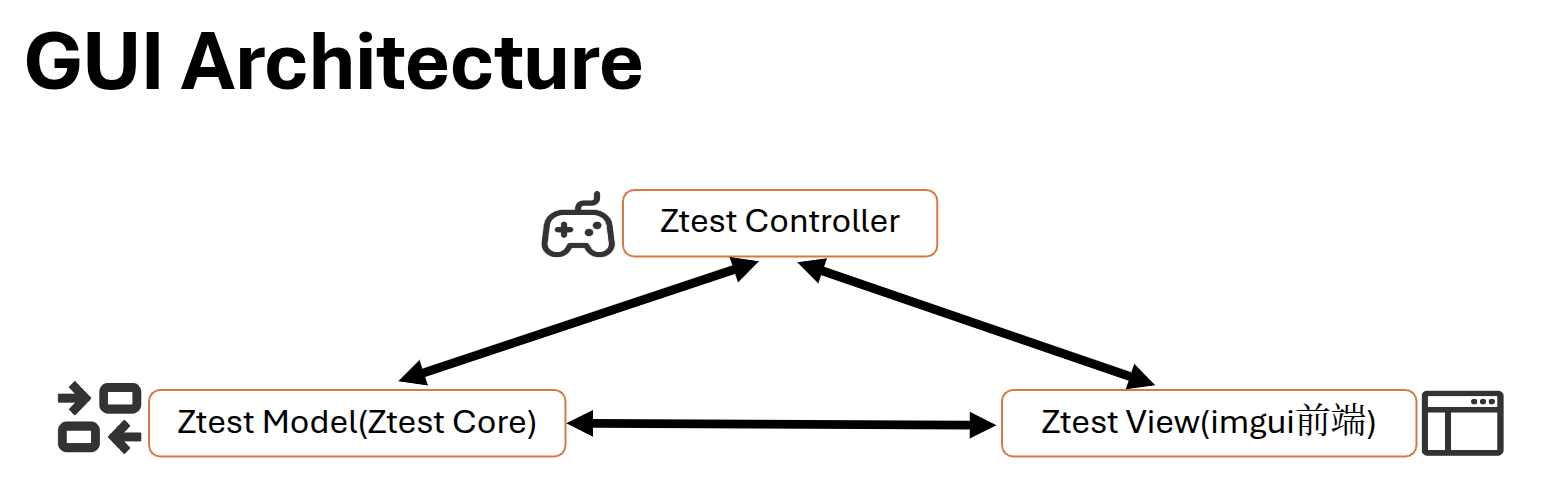
\includegraphics[width=0.8\textwidth]{img/guiarch.png} % 假设logo.png是学校标志的图片文件
    \caption{ ztest gui architecture}
    \label{fig:ztest gui architecture }
\end{figure}
\subsubsection{GUI框架}
GUI框架使用MCV架构开发,其中Model层负责数据处理,其中包含了对于Ztest core的进一步封装,View层负责界面绘制,主要是使用ImGui框架绘制,Controller层负责用户交互,将用户在UI界面上的点击和筛选等操作转换成对Model层和View层的调用,从而实现用户界面的更新和数据的更新。
\newpage
\begin{figure}[H]
    \centering
    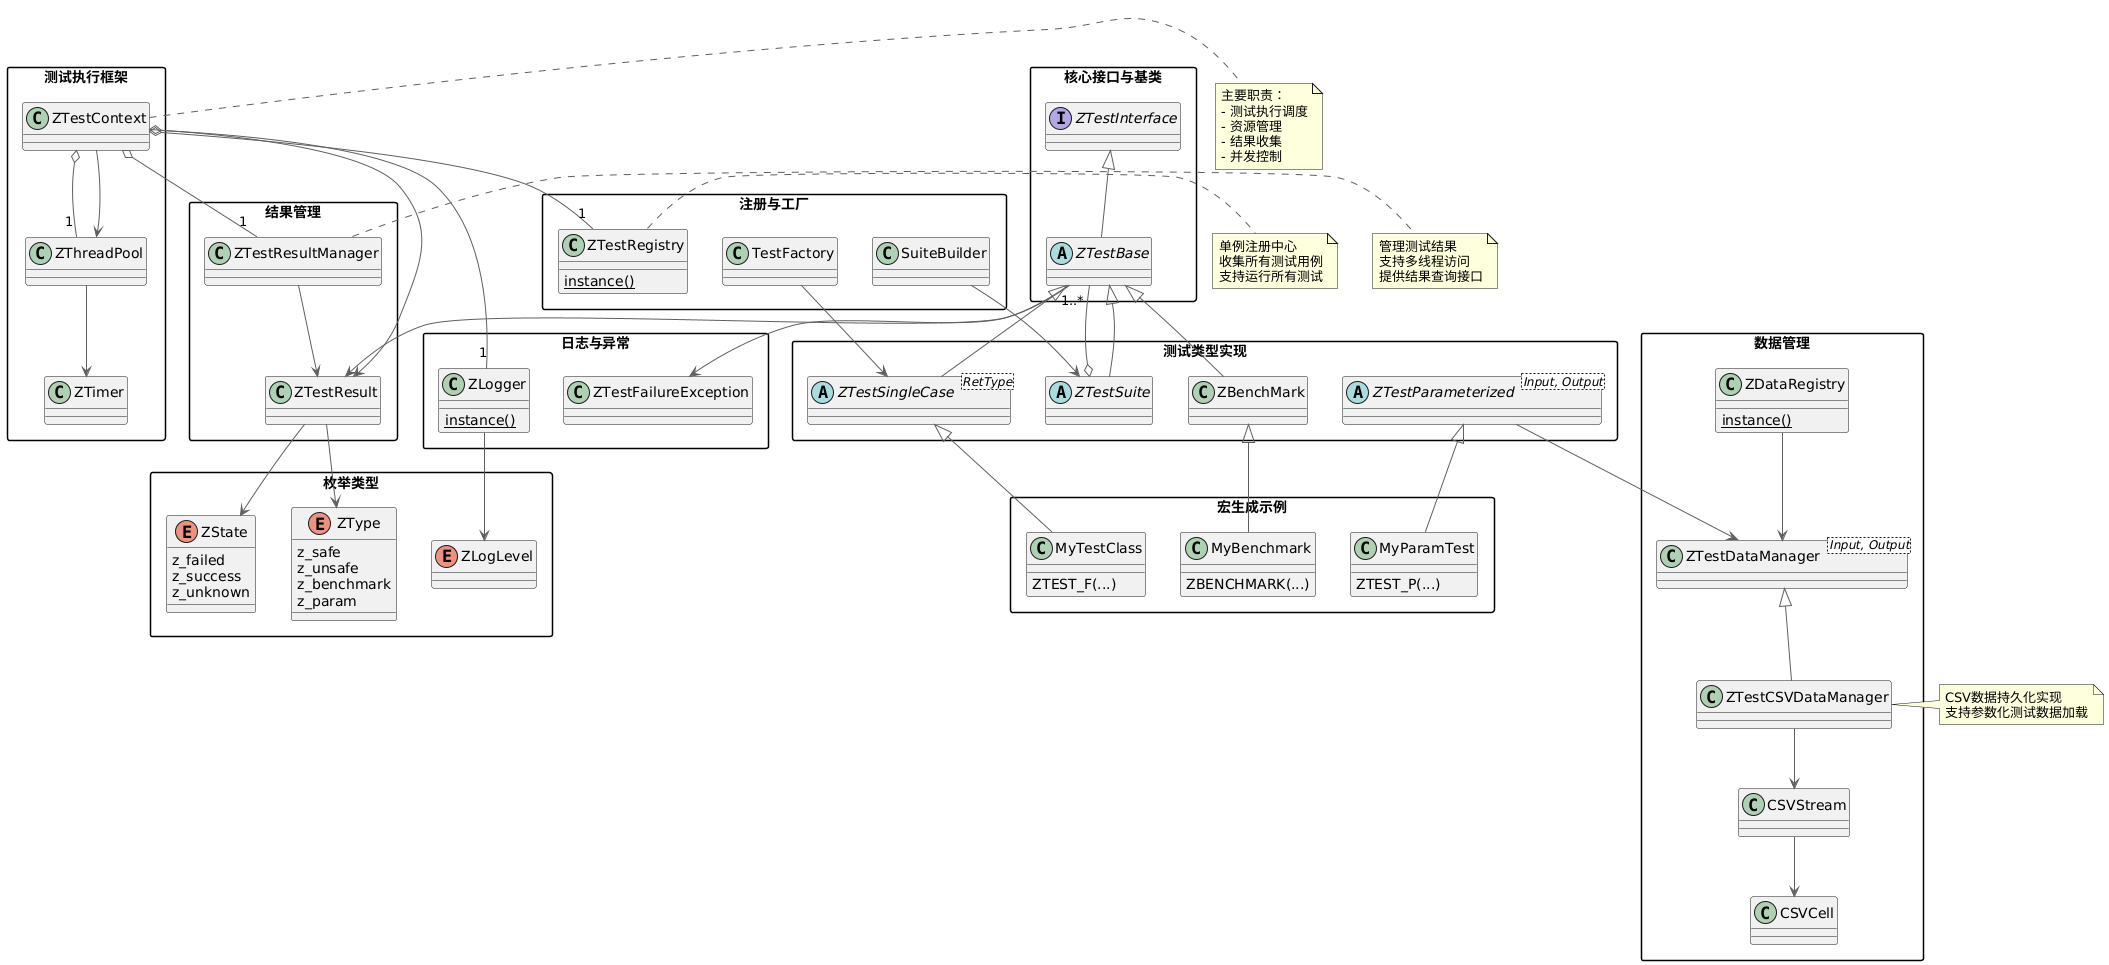
\includegraphics[angle=270,width=0.7\textwidth]{img/class.png} % 假设logo.png是学校标志的图片文件
    \caption{ ztest class}
    \label{fig:ztest class }
\end{figure}
\subsection{详细设计}
\subsubsection{测试定义相关类}
\begin{itemize}
    \item \texttt{ZTestBase} (ztest\_base.hpp): 抽象测试基类,封装通用属性与生命周期钩子。采用模板方法模式定义测试执行框架,通过虚函数表实现策略模式,利用钩子函数实现装饰器模式扩展。
    \item \texttt{ZTestSingleCase} (ztest\_singlecase.hpp): 单例测试实现,使用模板方法模式执行测试逻辑,配合TestFactory体现工厂模式,支持链式配置符合建造者模式特征。
    \item \texttt{ZBenchMark} (ztest\_benchmark.hpp): 基准测试类,继承ZTestBase并重写run()方法,通过迭代执行测试函数实现基准测试。
    \item \texttt{ZTestParameterized} (ztest\_parameterized.hpp): 参数化测试基类,采用组合模式封装测试数据,通过run()方法实现数据驱动测试框架。
\end{itemize}

\subsubsection{测试注册相关类}
\begin{itemize}
    \item \texttt{ZTestRegistry} (ztest\_registry.hpp): 单例模式实现的全局注册中心,管理测试用例集合并保障线程安全的注册/获取操作。
    \item \texttt{宏定义系统} (ztest\_macros.hpp): 通过宏定义实现语法糖,采用工厂模式自动生成测试类,利用命名连接技术实现自动化注册。
\end{itemize}

\subsubsection{测试执行相关类}
\begin{itemize}
    \item \texttt{ZTestContext} (ztest\_context.hpp): 测试执行上下文,采用策略模式根据测试类型选择执行策略,通过线程池模式实现并行测试执行。
    \item \texttt{ZThreadPool} (ztest\_thread.hpp): 线程池实现对象池模式,使用生产者-消费者模式管理任务队列,通过future/promise机制实现异步执行监控。
\end{itemize}

\subsubsection{结果管理相关类}
\begin{itemize}
    \item \texttt{ZTestResult} (ztest\_result.hpp): 值对象模式的测试结果类,封装测试状态、耗时等不可变数据。
    \item \texttt{ZTestResultManager} (ztest\_result.hpp): 单例模式实现的结果管理器,采用责任链模式处理结果存储与查询。
\end{itemize}

\subsubsection{报告生成相关类}
\begin{itemize}
    \item \texttt{ZLogger} (ztest\_logger.hpp): 多格式报告生成器,应用模板方法模式定义报告生成流程,支持HTML/JSON/JUnit报告格式。
\end{itemize}

\subsubsection{工具模块相关类}
\begin{itemize}
    \item \texttt{ZTimer} (ztest\_timer.hpp): RAII模式实现的计时器,封装时间测量功能。
    \item \texttt{ZDataRegistry} (ztest\_dataregistry.hpp): 数据缓存管理器,采用单例模式全局访问,通过LRU策略实现缓存淘汰。
\end{itemize}

\subsubsection{GUI模块相关类}
\begin{itemize}
    \item \texttt{ZTestModel} (gui.hpp): MVC架构中的Model层,采用观察者模式监听测试状态变化。
    \item \texttt{ZTestController} (gui.hpp): MVC架构中的Controller层,实现命令模式封装测试执行操作。
    \item \texttt{ZTestView} (gui.hpp): MVC架构中的View层,使用桥接模式分离界面元素与实现。
\end{itemize}

\section{编程进度}
\begin{table}[H]
    \centering
    \begin{tabular}{|l|l|}
        \toprule
        \textbf{任务阶段}                         & \textbf{计划}                       \\ \midrule
        \textbf{确定主题} 2024.04.26-2024.05.03   & 调查主题,提交提案。                        \\ \midrule
        \textbf{实现核心代码} 2024.05.03-2024.05.05 & 实现了GUI和Safe test和Unsafe test的执行逻辑 \\ \midrule
        \textbf{重大性能优化} 2024.05.05-2024.05.08 & 线程池优化                             \\ \midrule
        功能优化 2024.05.08-2024.05.11            & 完善JSON,HTML输出,JUnit格式输出,CI集成      \\ \midrule
        功能优化 2024.05.11-2024.05.13            & GUI引入了imgui Docking功能             \\ \midrule
        功能优化 2024.05.13-2024.05.15            & 增加CLI                             \\ \midrule
        \textbf{重大功能优化} 2024.05.15-2024.05.24 & 增加BENCHMARK测试                     \\ \midrule
        功能优化 2024.05.24-2024.05.25            & 增加了设备状态监测和可视化                     \\ \midrule
        \textbf{重大功能优化} 2024.05.25-2024.05.28 & 增加了参数化测试并增加了数据驱动                  \\ \midrule
        \textbf{重大性能优化} 2024.05.28-2024.06.02 & 增加了对数据的缓存和LRU缓存淘汰技术               \\ \midrule
        总结工作 2024.6.02-2024.06.08             & 跨平台移植 \& 报告撰写                     \\
        \bottomrule
    \end{tabular}
    \caption{编程进度}
\end{table}

\section{测试报告}
\subsection{功能测试}
% 在这里填写功能测试的内容

\subsection{系统测试}
% 在这里填写系统测试的内容

\section{个人总结}
% 在这里写下你的收获、建议等内容

\section{参考文献}
\begin{thebibliography}{99}
    \bibitem{ref1} [参考文献1]
    \bibitem{ref2} [参考文献2]
    % 根据实际情况继续添加
\end{thebibliography}

\end{document}修正